\definecolor{als}{RGB}{145 74 0}
\definecolor{ge}{RGB}{0 71 145}
\definecolor{ga}{RGB}{101 121 144}

% GNUPLOT: LaTeX picture with Postscript
\begingroup
  \makeatletter
  \providecommand\color[2][]{%
    \GenericError{(gnuplot) \space\space\space\@spaces}{%
      Package color not loaded in conjunction with
      terminal option `colourtext'%
    }{See the gnuplot documentation for explanation.%
    }{Either use 'blacktext' in gnuplot or load the package
      color.sty in LaTeX.}%
    \renewcommand\color[2][]{}%
  }%
  \providecommand\includegraphics[2][]{%
    \GenericError{(gnuplot) \space\space\space\@spaces}{%
      Package graphicx or graphics not loaded%
    }{See the gnuplot documentation for explanation.%
    }{The gnuplot epslatex terminal needs graphicx.sty or graphics.sty.}%
    \renewcommand\includegraphics[2][]{}%
  }%
  \providecommand\rotatebox[2]{#2}%
  \@ifundefined{ifGPcolor}{%
    \newif\ifGPcolor
    \GPcolorfalse
  }{}%
  \@ifundefined{ifGPblacktext}{%
    \newif\ifGPblacktext
    \GPblacktexttrue
  }{}%
  % define a \g@addto@macro without @ in the name:
  \let\gplgaddtomacro\g@addto@macro
  % define empty templates for all commands taking text:
  \gdef\gplfronttext{}%
  \gdef\gplfronttext{}%
  \makeatother
  \ifGPblacktext
    % no textcolor at all
    \def\colorrgb#1{}%
    \def\colorgray#1{}%
  \else
    % gray or color?
    \ifGPcolor
      \def\colorrgb#1{\color[rgb]{#1}}%
      \def\colorgray#1{\color[gray]{#1}}%
      \expandafter\def\csname LTw\endcsname{\color{white}}%
      \expandafter\def\csname LTb\endcsname{\color{black}}%
      \expandafter\def\csname LTa\endcsname{\color{black}}%
      \expandafter\def\csname LT0\endcsname{\color[rgb]{1,0,0}}%
      \expandafter\def\csname LT1\endcsname{\color[rgb]{0,1,0}}%
      \expandafter\def\csname LT2\endcsname{\color[rgb]{0,0,1}}%
      \expandafter\def\csname LT3\endcsname{\color[rgb]{1,0,1}}%
      \expandafter\def\csname LT4\endcsname{\color[rgb]{0,1,1}}%
      \expandafter\def\csname LT5\endcsname{\color[rgb]{1,1,0}}%
      \expandafter\def\csname LT6\endcsname{\color[rgb]{0,0,0}}%
      \expandafter\def\csname LT7\endcsname{\color[rgb]{1,0.3,0}}%
      \expandafter\def\csname LT8\endcsname{\color[rgb]{0.5,0.5,0.5}}%
    \else
      % gray
      \def\colorrgb#1{\color{black}}%
      \def\colorgray#1{\color[gray]{#1}}%
      \expandafter\def\csname LTw\endcsname{\color{white}}%
      \expandafter\def\csname LTb\endcsname{\color{black}}%
      \expandafter\def\csname LTa\endcsname{\color{black}}%
      \expandafter\def\csname LT0\endcsname{\color{black}}%
      \expandafter\def\csname LT1\endcsname{\color{black}}%
      \expandafter\def\csname LT2\endcsname{\color{black}}%
      \expandafter\def\csname LT3\endcsname{\color{black}}%
      \expandafter\def\csname LT4\endcsname{\color{black}}%
      \expandafter\def\csname LT5\endcsname{\color{black}}%
      \expandafter\def\csname LT6\endcsname{\color{black}}%
      \expandafter\def\csname LT7\endcsname{\color{black}}%
      \expandafter\def\csname LT8\endcsname{\color{black}}%
    \fi
  \fi
    \setlength{\unitlength}{0.0500bp}%
    \ifx\gptboxheight\undefined%
      \newlength{\gptboxheight}%
      \newlength{\gptboxwidth}%
      \newsavebox{\gptboxtext}%
    \fi%
    \setlength{\fboxrule}{0.5pt}%
    \setlength{\fboxsep}{1pt}%
\begin{picture}(5000.00,2000.00)%
    \gplgaddtomacro\gplfronttext{%
      \colorrgb{0.15,0.15,0.15}%

      \put(900,2100){\makebox(0,0){\strut{}{\color{ge}{\rule[0.6mm]{0.6cm}{1.0mm}}} \footnotesize CBGL }}
      \put(2500,2100){\makebox(0,0){\strut{}{\color{ga}{\rule[0.6mm]{0.6cm}{1.0mm}}} \footnotesize $\mathcal{H}_1($$k$$=$$10$$)$}}
      \put(4200,2100){\makebox(0,0){\strut{}{\color{als}{\rule[0.6mm]{0.6cm}{1.0mm}}} \footnotesize ALS [1]}}

      \put(468,250){\makebox(0,0)[r]{\strut{}\footnotesize $0\%$}}%
      \colorrgb{0.15,0.15,0.15}%
      \put(468,650){\makebox(0,0)[r]{\strut{}\footnotesize $25\%$}}%
      \colorrgb{0.15,0.15,0.15}%
      \put(468,1050){\makebox(0,0)[r]{\strut{}\footnotesize $50\%$}}%
      \colorrgb{0.15,0.15,0.15}%
      \put(468,1484){\makebox(0,0)[r]{\strut{}\footnotesize $\textcolor{ga}{77.2}\%$}}%
      \colorrgb{0.15,0.15,0.15}%
      \put(468,1835){\makebox(0,0)[r]{\strut{}\footnotesize $\textcolor{ge}{99.1\%}$}}%
      \colorrgb{0.15,0.15,0.15}%
      %\put(500,-20){\makebox(0,0){\strut{}\footnotesize $0.00047988$}}%
      \colorrgb{0.15,0.15,0.15}%
      \put(936,-20){\makebox(0,0){\strut{}\footnotesize $0.01$}}%
      \colorrgb{0.15,0.15,0.15}%
      \put(1497,-20){\makebox(0,0){\strut{}\footnotesize $0.50$}}%
      \colorrgb{0.15,0.15,0.15}%
      %\put(1927,-20){\makebox(0,0){\strut{}\footnotesize $10.0$}}%
      \colorrgb{0.15,0.15,0.15}%
      \put(2074,-20){\makebox(0,0){\strut{}\footnotesize $27.9$}}%
    }%
    \gplgaddtomacro\gplfronttext{%
      \colorrgb{0.15,0.15,0.15}%
      %\put(1287,-350){\makebox(0,0){\strut{}\footnotesize Outliers locational threshold $\delta_{\bm{l}}$ [m]}}%
      \put(1287,-350){\makebox(0,0){\strut{}\footnotesize Location error $\delta_{\bm{l}}$ [m]}}%
    }%
    \gplgaddtomacro\gplfronttext{%
      \colorrgb{0.15,0.15,0.15}%
      \put(2893,250){\makebox(0,0)[r]{\strut{}\footnotesize $0\%$}}%
      \colorrgb{0.15,0.15,0.15}%
      \put(2893,630){\makebox(0,0)[r]{\strut{}\footnotesize $25\%$}}%
      \colorrgb{0.15,0.15,0.15}%
      \put(2893,869){\makebox(0,0)[r]{\strut{}\footnotesize $\textcolor{ga}{37.5\%}$}}%
      \colorrgb{0.15,0.15,0.15}%
      \put(2893,1760){\makebox(0,0)[r]{\strut{}\footnotesize $\textcolor{ge}{94.4\%}$}}%
      \colorrgb{0.15,0.15,0.15}%
      %\put(2925,-20){\makebox(0,0){\strut{}\footnotesize $4.1313e-05$}}%
      \colorrgb{0.15,0.15,0.15}%
      \put(4114,-20){\makebox(0,0){\strut{}\footnotesize $2\pi/100$}}%
      \colorrgb{0.15,0.15,0.15}%
      \put(4749,-20){\makebox(0,0){\strut{}\footnotesize $\pi$}}%
    }%
    \gplgaddtomacro\gplfronttext{%
      \colorrgb{0.15,0.15,0.15}%
      %\put(3837,-350){\makebox(0,0){\strut{}\footnotesize Outliers angular threshold $\delta_{\theta}$ [rad]}}%
      \put(3837,-350){\makebox(0,0){\strut{}\footnotesize Orientation error $\delta_{\theta}$ [rad]}}%
    }%
    \put(0,0){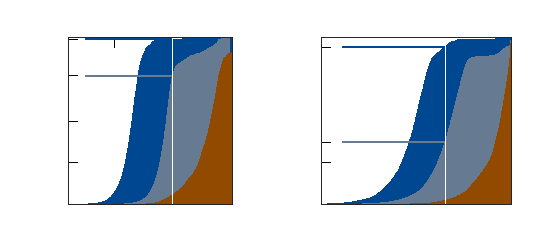
\includegraphics{figures/12/awesomeness}}%
    \gplfronttext
  \end{picture}%
\endgroup
